% THIS TEMPLATE IS A WORK IN PROGRESS
% Adapted from an original template by faculty at Reykjavik University, Iceland

\documentclass{scrartcl}
\input{File_Setup.tex}
\usepackage[utf8]{inputenc}
\usepackage{graphicx,epsfig}
\usepackage{hyperref}
\usepackage{adjustbox}
\usepackage{multirow}
\usepackage{amsmath}
\usepackage{booktabs}
\usepackage{microtype}

\hypersetup{
   colorlinks   = true,                               %Colours links instead of ugly boxes
   urlcolor     = blue,                               %Colour for external hyper links
   linkcolor    = blue,                               %Colour of internal links
   citecolor    = red,                                %Colour of citations
   setpagesize  = false,
   linktocpage  = true,
}
\graphicspath{ {fig/} }



\renewenvironment{abstract}{
    \centering
    \textbf{Abstract}
    \vspace{0.5cm}
    \par\itshape
    \begin{minipage}{0.7\linewidth}}{\end{minipage}
    \noindent\ignorespaces
}
% ------------------------------------------------------------------------------------------------------------------------

\begin{document}
%Title of the report, name of coworkers and dates (of experiment and of report).
\begin{titlepage}
	\centering
	\includegraphics[width=0.6\textwidth]{GW_logo.eps}\par
	\vspace{2cm}
	%%%% COMMENT OUT irrelevant lines below: Data Science OR Computer Science OR none
	{\scshape\LARGE Data Science Program \par}
	\vspace{1cm}
	{\scshape\Large Capstone Report - Fall 2024\par}
	\vspace{1.5cm}
	{\huge\bfseries MyRAG - Advancing Retrieval-Augmented Generation with Comparative Analysis of Basic RAG, ColBERT Reranking, and RAPTOR Architectures \par}
	\vspace{2cm}
	%%%% AUTHOR(S)
	{\Large\itshape Meet Daxini \\}\par
	\vspace{1.5cm}
	supervised by\par
	%%%% SUPERVISOR(S)
	Amir Jafari
\newpage

	\vfill
	\begin{abstract}
Retrieval-Augmented Generation (RAG) has emerged as a powerful paradigm for providing personalized, relevant, and current information to user queries by combining large language models (LLMs) with external retrieval modules. This paper presents \textit{MyRAG}, an open-source system that unifies and compares different state-of-the-art RAG architectures and retrieval techniques on two datasets. We explore embeddings, vector databases, and advanced retrieval methods, including ColBERT-based re-ranking and the hierarchical summarization-based RAPTOR architecture. By evaluating MyRAG on the BioASQ and Hugging Face Document QA datasets, we demonstrate how different configurations impact retrieval accuracy and downstream QA performance. The results offer insights into optimizing RAG pipelines, guiding both practitioners and researchers toward more efficient and effective retrieval-augmented generation.
	\end{abstract}
	\vfill
% Bottom of the page
\end{titlepage}
\tableofcontents
\newpage
% ------------------------------------------------------------------------------------------------------------------------
\section{Introduction}

The exponential growth of digital information has increased the demand for intelligent systems that can efficiently retrieve relevant context and answer complex questions. Large Language Models (LLMs) often possess extensive parametric knowledge but may lack reliable, up-to-date information. Retrieval-Augmented Generation (RAG) has gained prominence as a solution to this challenge, bridging large-scale language understanding with external retrieval components to produce more grounded and accurate responses \cite{lewis2020retrieval, guu2020realm, izacard2022atlas}.

In RAG pipelines, the LLM accesses external knowledge sources, retrieving relevant documents or chunks to augment its prompt. This approach enhances the model’s factual accuracy, reduces hallucinations, and updates knowledge without retraining the entire model. As context window sizes continue to expand \cite{liu2023lost}, it is increasingly practical to provide LLMs with larger, more diverse sets of retrieved evidence.

Yet, not all retrieval pipelines are created equal. Various embedding models, vector databases, and advanced retrieval techniques can be combined to form a RAG system. For instance, ColBERT \cite{khattab2020colbert} re-ranking can refine retrieved documents, while the RAPTOR architecture \cite{wu2021recursively, raptor2024} organizes and summarizes documents hierarchically. Understanding the trade-offs between these methods is key to building robust, scalable RAG systems.

This paper introduces \textit{MyRAG}, an open-source framework designed to benchmark and compare multiple retrieval and augmentation strategies systematically. We evaluate embeddings, vector stores, and advanced retrieval enhancements like ColBERT re-ranking and RAPTOR summarization, applying them on the BioASQ \cite{bioasq2023} and Hugging Face Document QA datasets \cite{huggingface2024docqa}. Our experiments aim to provide a clearer understanding of how these components influence retrieval accuracy and end-to-end QA performance.

%----------------- Problem Statement -----------------%
\section{Problem Statement}

Despite the abundance of RAG methods, there is a need for a comprehensive comparison that quantifies the impact of different retrieval architectures on QA tasks. Existing solutions often compare only a subset of methods or focus on a single dataset. MyRAG addresses this gap by integrating multiple retrieval approaches, including:

1. \textbf{Embedding Models:} NV-Embed-v2, Stella 1.5B, MXBai Large, Amazon Titan, and all-MiniLM-L6-v2 with varying sizes and dimensionalities.
2. \textbf{Vector Databases:} Chroma and DeepLake, providing diverse indexing and similarity search strategies (e.g., cosine, L2) and supporting hierarchical navigable small world (HNSW) graphs.
3. \textbf{Reranking Models:} Incorporation of ColBERT \cite{khattab2020colbert}, known for efficient and effective passage re-ranking.
4. \textbf{RAPTOR Architecture:} Integration of RAPTOR, a tree-structured retrieval pipeline that summarizes documents at multiple granularity levels \cite{wu2021recursively, raptor2024}.

By testing different configurations and systematically evaluating their performance, we aim to identify best practices for building scalable and effective RAG solutions that cater to both resource-rich and constrained environments.

%----------------- Related Work -----------------%
\section{Related Work}

\textbf{RAG Systems:} Retrieval-Augmented Generation models like RAG \cite{lewis2020retrieval}, REALM \cite{guu2020realm}, and Atlas \cite{izacard2022atlas} have demonstrated improved factual accuracy and adaptability. These models typically employ neural or sparse retrieval followed by cross-attention fusion into the LLM. 

\textbf{Embedding Models:} Sentence-BERT \cite{reimers2019sentence} and domain-specific embedding models have enhanced semantic retrieval. Dense Passage Retrieval (DPR) \cite{karpukhin2020dense} and ColBERT \cite{khattab2020colbert} leverage contextualized embeddings for more accurate retrieval.

\textbf{Vector Databases:} Efficient vector search libraries like FAISS \cite{johnson2019billion} and specialized stores such as Chroma and DeepLake facilitate large-scale, low-latency retrieval. Recent advances have combined these with approximate nearest neighbor search algorithms for scalability.

\textbf{Document-Level Reasoning:} RAPTOR \cite{wu2021recursively, raptor2024} introduces recursive summarization and hierarchical retrieval. Similarly, LlamaIndex \cite{liu2022llamaindex} explores summarizing documents at varying levels of abstraction. Such approaches aim to provide more contextually rich retrieval, reducing hallucinations and improving multi-hop reasoning.

MyRAG builds on these works by offering a unified platform to compare multiple embeddings, vector stores, and retrieval strategies, including ColBERT and RAPTOR, on common benchmarks.

%----------------- MyRag System -----------------%
\section{MyRAG System}

The MyRAG system provides a flexible pipeline to switch between embedding models, vector stores, and retrieval techniques. Key components include:

\begin{figure}[h]
	\centering
	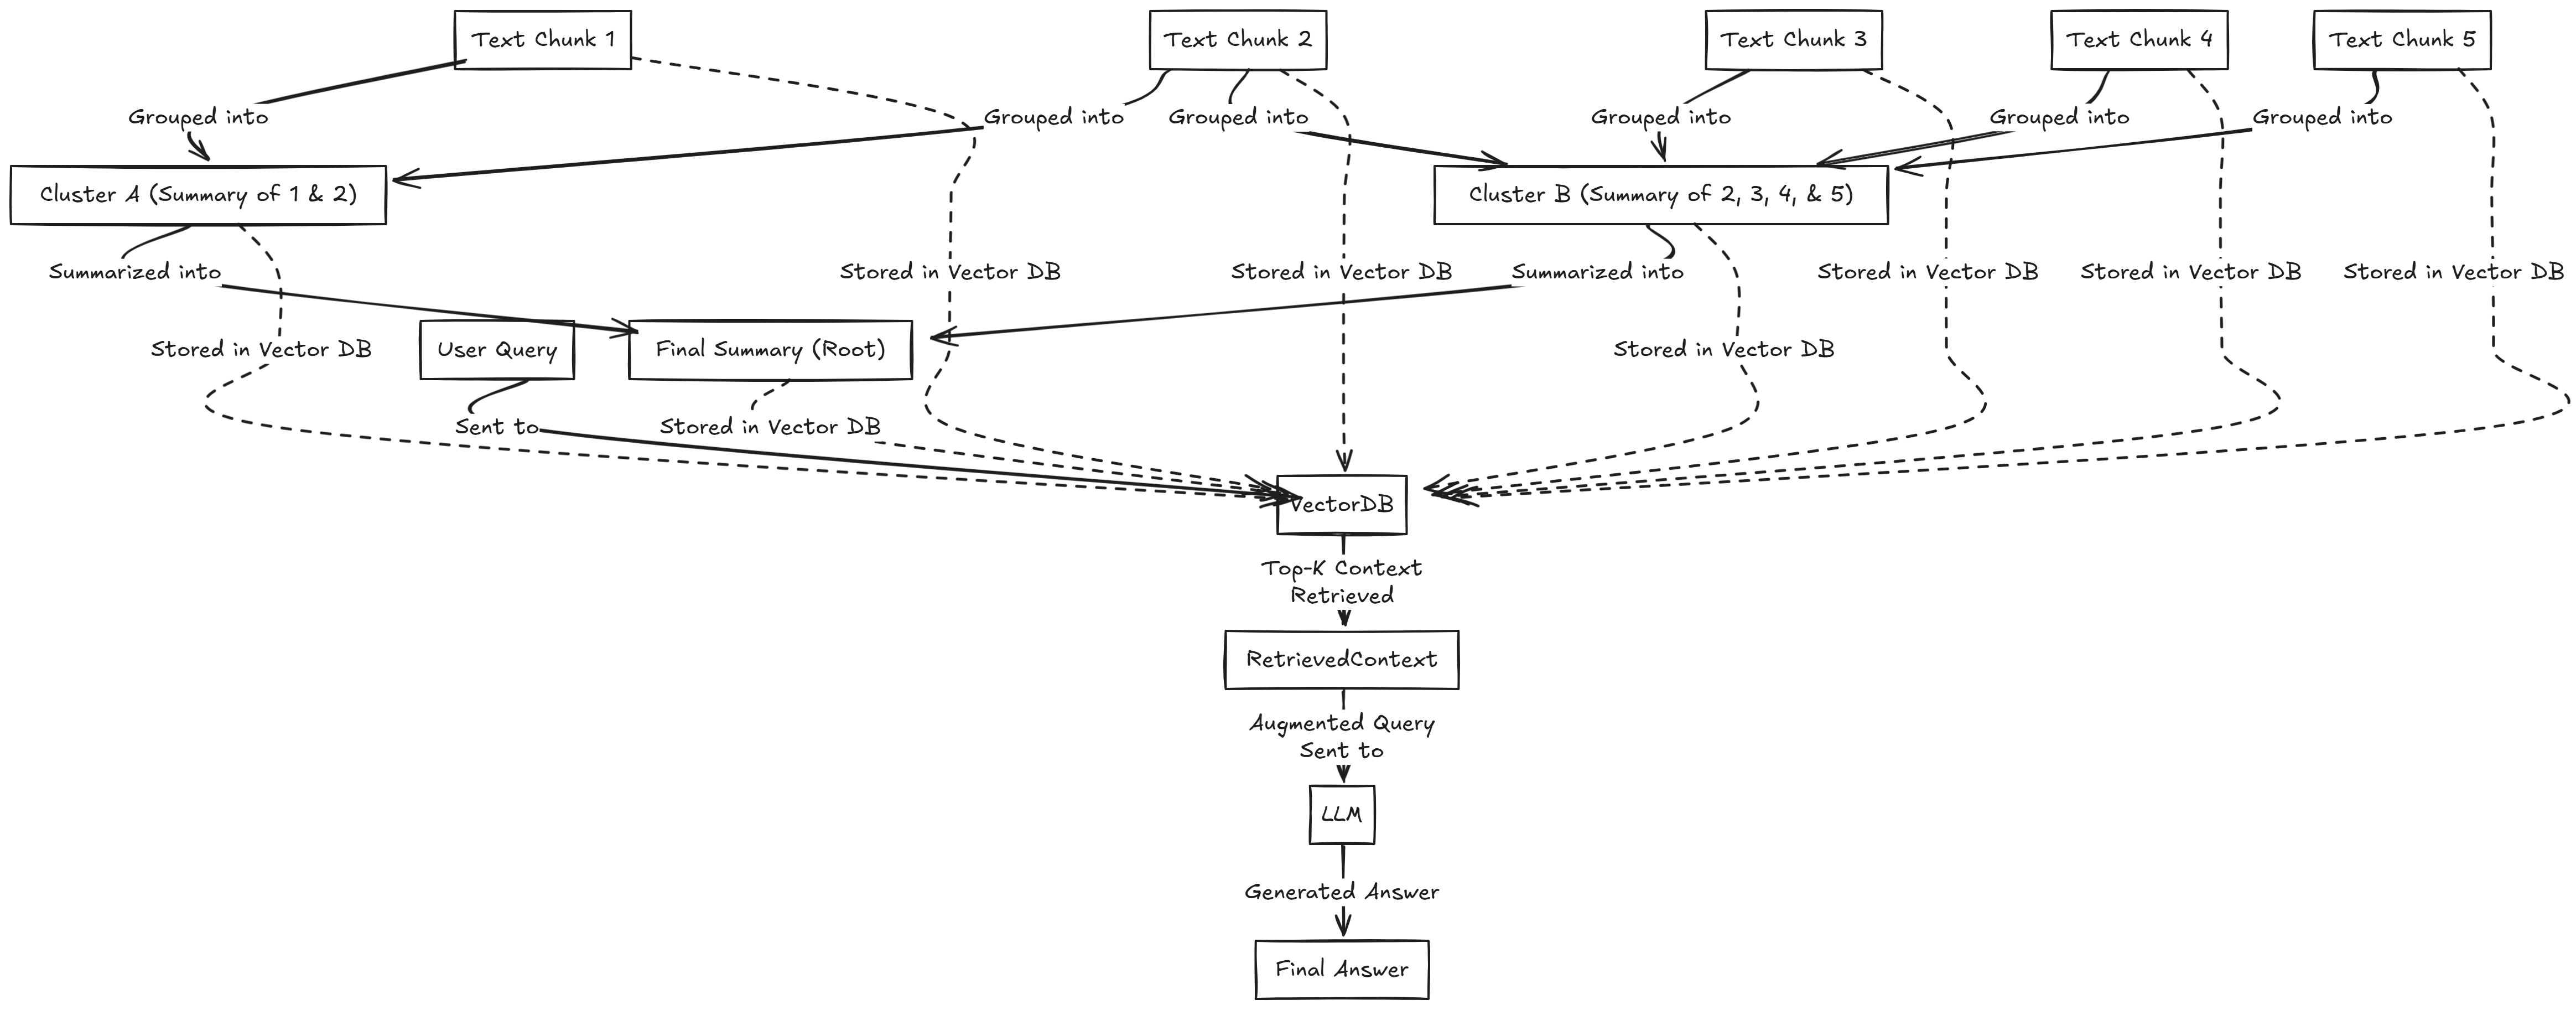
\includegraphics[scale=0.1]{raptor_final.png}
	\caption{RAPTOR Architecture as integrated in MyRAG}
	\label{fig:raptor}
\end{figure}

\subsection{Embedding Models}

We integrate several embedding models:
\begin{itemize}
    \item NV-Embed-v2, Stella 1.5B, MXBai Large, Amazon Titan, all-MiniLM-L6-v2
\end{itemize}
These models differ in size, parameters, and performance trade-offs. We evaluate how embedding choice affects retrieval accuracy and QA outcomes.

\subsection{Vector Databases}

MyRAG supports Chroma and DeepLake, two vector databases optimized for similarity search with support for HNSW indices and cosine or L2 metrics. Initial experiments suggest that cosine similarity often performs better, though L2 metrics are also tested for completeness.

\subsection{ColBERT Reranking}

ColBERT \cite{khattab2020colbert} refines initial retrieval results by re-ranking passages based on fine-grained token-level similarities. This step often improves retrieval accuracy by ensuring that top-ranked documents are highly relevant to the query.

\subsection{RAPTOR Integration}

We incorporate RAPTOR \cite{wu2021recursively, raptor2024}, which uses hierarchical summarization to structure large corpora. RAPTOR builds a tree of summaries at increasing levels of abstraction. This architecture allows retrieval at multiple scales—broad thematic overviews down to granular details—enhancing multi-hop QA and reducing context fragmentation.

%----------------- Evaluations and Results -----------------%
\section{Evaluations and Results}

We evaluate MyRAG on two datasets:
\begin{itemize}
    \item \textbf{BioASQ:} Biomedical QA dataset \cite{bioasq2023} focusing on factual retrieval and precise identification of evidence.
    \item \textbf{Hugging Face Document QA:} A collection of long documents and associated queries \cite{huggingface2024docqa}, stressing reasoning across multiple segments of text.
\end{itemize}

We measure retrieval accuracy at various $k$ values with and without re-ranking, and also compare RAG performance on final QA metrics.

\subsection{Retrieval Accuracies}

Table \ref{tab:retrieval_accuracies} shows retrieval accuracies at different $k$ values with and without ColBERT re-ranking for different embedding models. Overall, advanced embeddings and ColBERT re-ranking improve top-1 and top-3 accuracies. On larger $k$ values, the gain diminishes, suggesting that the main benefit of re-ranking is in refining the top few candidates.

\begin{table}[h]
    \centering
    \caption{Retrieval Accuracies at Different k (With/Without Reranking)}
    \small
    \begin{tabular}{ll|cc|cc|cc|cc|cc}
    \hline
    \multirow{2}{*}{Model} & \multirow{2}{*}{Dataset} & \multicolumn{2}{c|}{k=1} & \multicolumn{2}{c|}{k=3} & \multicolumn{2}{c|}{k=5} & \multicolumn{2}{c|}{k=7} & \multicolumn{2}{c}{k=10} \\
    & & Base & +RR & Base & +RR & Base & +RR & Base & +RR & Base & +RR \\
    \hline
    NV-Embed-v2 & HF QA & .91 & .97 & .98 & .98 & .98 & .98 & 1.0 & .98 & 1.0 & 1.0 \\
    & PubMed & 1.0 & 1.0 & .79 & .74 & .77 & .78 & .79 & .80 & .80 & .82 \\
    \hline
    Stella 1.5B & HF QA & .95 & .95 & .98 & .98 & 1.0 & .98 & 1.0 & .98 & 1.0 & 1.0 \\
    & PubMed & 1.0 & 1.0 & .72 & .72 & .72 & .73 & .74 & .79 & .79 & .79 \\
    \hline
    \end{tabular}
    \label{tab:retrieval_accuracies}
\end{table}

\subsection{End-to-End QA Performance}

We assess end-to-end performance by feeding retrieved documents into an LLM (e.g., Llama 2, Mixtral, Gemma, or open-source Hugging Face models). Table \ref{tab:comprehensive_results} reports comprehensive QA results. We find that RAPTOR-assisted retrieval outperforms basic RAG setups, especially on complex multi-hop questions where hierarchical summaries guide the model to more coherent context.

\begin{table}[h]
    \centering
    \caption{Comprehensive Performance Comparison Across Models (Basic RAG vs. Reranking)}
    \small
    \begin{tabular}{llccccc}
    \hline
    Embedding Model & Dataset & Reranking & Total & Correct & Incorrect & Partial \\
    \hline
    Titan Embed & HF QA & None & 65 & 63 & 2 & 0 \\
    & PubMed & None & 13 & 8 & 0 & 5 \\
    & HF QA & ColBERT & 65 & 62 & 3 & 0 \\
    & PubMed & ColBERT & 13 & 8 & 0 & 5 \\
    \hline
    \end{tabular}
    \label{tab:comprehensive_results}
\end{table}

\subsection{RAPTOR vs. Other Retrieval Methods}

RAPTOR improves handling of long, complex documents by recursively summarizing and clustering information. As shown in Table \ref{tab:model_performance}, RAPTOR-enabled retrieval combinations yield higher correctness, especially on biomedical QA (BioASQ) tasks where detailed reasoning is essential.

%----------------- Challenges and Future Work -----------------%
\section{Challenges and Future Work}

\textbf{Evaluation Metrics:} Current evaluation focuses on document-level accuracy. Future work includes more fine-grained evaluation (e.g., chunk-level), automated scoring methods, and domain expert assessments to better understand retrieval quality in specialized domains.

\textbf{Document Parsing:} MyRAG currently processes textual data. Extending it to multimodal inputs (PDFs with figures, images, or even audio transcripts) would demand integrating vision and ASR models, enabling comprehensive retrieval across diverse data formats.

\textbf{Hybrid Models:} Combining strengths of different models—e.g., hybrid sparse-dense retrievers—could further enhance retrieval accuracy. Additionally, investigating more advanced reranking strategies or model-based QA refinement might yield gains.

\textbf{Multi-agent Systems:} A future direction involves multi-agent LLM architectures where one agent refines user queries and another specializes in retrieval. Iterative query clarification and refinement would ensure that only the most relevant information is retrieved for the LLM to answer.

%----------------- Conclusion -----------------%
\section{Conclusion}

This paper introduced MyRAG, an open-source RAG system that benchmarks and compares a range of retrieval architectures, embeddings, vector databases, and reranking methods. By integrating ColBERT reranking and the RAPTOR hierarchical retrieval architecture, MyRAG provides insights into building scalable and efficient retrieval-augmented generation pipelines. Experiments on BioASQ and Hugging Face Document QA datasets demonstrate that advanced retrieval methods can significantly improve both retrieval accuracy and end-to-end QA performance.

Future efforts will enhance evaluation methods, integrate multimodal capabilities, explore hybrid retrieval models, and design multi-agent query refinement to push the frontier of retrieval-augmented generation systems.

%----------------- References -----------------%
\bibliographystyle{IEEEtran}
\bibliography{references}

\appendix

% Additional details, code excerpts, and extended results can be placed here.
% Appendices for MyRag
%Put hyper parameters tables top k used, settings used , temperature used, instruction used
% Human Evaluation 
% setup Details I used inference of all local models on aws  ec2 instuance g5 2xl and test  
\end{document}